%%%%%%%%%%TO FORMAT A PREPRINT FOR A PCI%%%%%%%%%%%%%%%%
%%%%%%%%%%%%%%%%%%%%%%%%%%%%%%%%%%%%%%%%%%%%%%

\documentclass{article}

\usepackage[letterpaper, margin=1in]{geometry}

\usepackage{lineno}
\linenumbers
\usepackage{titlesec}
%\usepackage[none]{hyphenat} % use only if there is a problem
% Use Unicode characters
\usepackage[utf8]{inputenc}
% Clean citations with biblatex
\usepackage[
backend=biber,
style=numeric
]{biblatex}

\addbibresource{zotero.bib}

% Highlighting
\usepackage{color}
\usepackage{soul}
\usepackage{xurl}

% tables
\usepackage{longtable,booktabs,array}
\usepackage{multirow}
\usepackage{afterpage}

% figures
\usepackage{wrapfig}
\usepackage{lscape}
\usepackage{rotating}
\usepackage{graphicx}
\graphicspath{assets}
\usepackage{times}

\newenvironment{sciabstract}{%
\begin{quote} \bf}
{\end{quote}}

% Include your paper's title here

\title{Gut microbes and their genes are associated with cognition and neuroanatomy in children}

% Place the author information here.  Please hand-code the contact
% information and notecalls; do *not* use \footnote commands.  Let the
% author contact information appear immediately below the author names
% as shown.  We would also prefer that you don't change the type-size
% settings shown here.

\author{%
    \parbox{\linewidth}{\centering
        Kevin S. Bongham,$^{1}$
        Guilherme Fahur Botino,$^{1}$
        Shelley Hoeft McCann,$^{1}$
        Jennifer Beauchemin,$^{2}$
        Elizabeth Weisse,$^{3}$
        Fatoumata Barry,$^{2}$
        Rosa Cano Lorente,$^{2}$
        The RESONANCE Consortium,
        Jonathan O'Muircheartaigh,$^{3}$
        Curtis Huttenhower,$^{4}$
        Muriel Bruchhage,$^{3}$
        Viren D’Sa,$^{2}$
        Sean Deoni,$^{2}$
        Vanja Klepac-Ceraj$^{1\ast}$
    }
\\
\normalsize{$^{1}$Department of Biological Sciences, Wellesley College,}\\
\normalsize{106 Central St, Wellesley, MA \hl{02---}, USA}\\
\normalsize{$^{2}$Rhode Island Hospital, Providence, RI, \hl{00000} USA}\\
\normalsize{$^{3}$\hl{Locations for Muriel, Jonathan, Sean}}\\
\normalsize{$^{4}$\hl{Department of Biostatistics, Harvard T.H. Chan School of Public Health}}\\
\normalsize{\hl{address of HSPH...}}
\\
\normalsize{$^\ast$To whom correspondence should be addressed; E-mail:  vklepacc@wellesley.edu.}
}

% Include the date command, but leave its argument blank.

\date{}


\begin{document}

\baselineskip24pt

% Make the title.

\maketitle 

\begin{abstract}
The gastrointestinal tract, its resident microorganisms and the central
nervous system are connected by biochemical signaling, also known as
"microbiome-gut-brain-axis." Both the human brain and the gut microbiome
have critical developmental windows in the first three years of life,
raising the possibility that their development is co-occurring and
likely co-dependent. Emerging evidence implicates gut microorganisms and
microbiota composition in cognitive outcomes and neurodevelopmental
disorders (e.g., autism and anxiety), but the influence of gut microbial
metabolism on typical neurodevelopment has not been explored in detail.
We investigated the relationship of the microbiome with the neuroanatomy
and cognitive function of 361 healthy children, demonstrating that
differences in gut microbial taxa and gene functions are associated with
overall cognitive function as well as with differences in the size of
multiple brain regions. Using a combination of multivariate linear
models and machine learning (ML) models, we showed that many species,
including \emph{Gordonibacter pamelae} and \emph{Blautia wexlerae}, were
significantly associated with higher cognitive function, while some
species such as \emph{Ruminococcus gnavus} were more commonly found in
children with low cognitive scores regardless of age or maternal
education. Microbial genes for enzymes involved in the metabolism of
neuroactive compounds, particularly short-chain fatty acids such as
glutamate and propionate, were also associated with cognitive function.
In addition, ML models were able to use microbial taxa to predict the
volume of brain regions, with particular taxa often dominating the
feature importance metric for individual brain regions, such as \emph{B.
wexlerae} being the most dominant for the parahippocampal region or
GABA-producing \emph{Bacteroidetes ovatus} for left accumbens. These
findings provide potential biomarkers of neurocognition and may lead to
the future development of targets for early detection and early
intervention.
\end{abstract}

%%%%%%%%%%%%%%%%%%%%%%%%%%%% Text of the preprint %%%%%%%%%%%%%%%%%%%%%%%%%%%%%%
%%%%%%%%%%%%%%%%%%%%%%%%%%%%%%%%%%%%%%%%%%%%%%%%%%%%%%%%%%%%%%%%%%%%%%%%%%%%%%%%
% use \emph{} for italics and \parencite{} to cite a reference and \ref{XX} to cite the \label{XX}
% use \\ and a blank line to mark the end of paragraph and starting of a new one

\section*{Introduction}

The gut and the brain are intimately linked. Signals from the brain
reach the gut through the autonomic nervous system and the endocrine
system, and the gut can communicate with the brain through the vagus
nerve and through endocrine and immune (cytokine) signaling molecules
\cite{cerdoEarlyNutritionGut2019,pronovostPerinatalInteractionsMicrobiome2019,sharonCentralNervousSystem2016,togniniGutMicrobiotaPotential2017}
In addition, the products of microbial metabolism generated in the gut can
influence the brain, both indirectly by stimulating the enteric nervous
and immune systems, as well as directly through molecules that enter
circulation and cross the blood-brain barrier. Causal links between the
gut microbiome and neural development, particularly atypical
development, are increasingly being identified
\cite{spichakMiningMicrobesMental2021}.
Both human epidemiology and animal models point to the effects
of gut microbes on the development of autism spectrum disorder
\cite{laueProspectiveAssociationsInfant2020,wanUnderdevelopmentGutMicrobiota2021}
and particular microbial taxa have been associated with depression
\cite{mayneris-perxachsMicrobiotaAlterationsProline2022,valles-colomerNeuroactivePotentialHuman2019}
and Alzheimer's disease
\cite{fungInteractionsMicrobiotaImmune2017,kimProbioticSupplementationImproves2021}.
But information about this "microbiome-gut-brain
axis" in normal neurocognitive development remains lacking,
particularly early in life.

The first years of life are critical developmental windows for both the
microbiome and the brain
\cite{laueDevelopingMicrobiomeBirth2022}.
Fetal development \emph{in utero} is believed to be mostly sterile, but
is rapidly seeded at birth through contact with the birth canal (if
birthed vaginally), caregivers, food sources (breastmilk or formula),
and other environmental sources such as antibiotics
\cite{backhedDynamicsStabilizationHuman2015,bokulichAntibioticsBirthMode2016}.
The early microbiome is characterized by low microbial
diversity, rapid succession and evolution, and domination by
Actinobacteria, particularly the genus \emph{Bifidobacterium},
Bacteroidetes, especially \emph{Bacteroides}, and Proteobacteria
\cite{koenigSuccessionMicrobialConsortia2011}.
Many of these microbes have specialized metabolic capabilities
for digesting human breast milk, such as \emph{Bifidobacterium infantis}
and \emph{Bacteroides fragilis}
\cite{selaGenomeSequenceBifidobacterium2008}.
Upon the introduction of solid foods, the gut
microbiome undergoes another categorical transformation, with most taxa
of the infant microbiome being replaced by taxa more reminiscent of
adult microbiomes
\cite{backhedDynamicsStabilizationHuman2015}.
Many prior studies have focused on either infant microbiomes or
adult microbiomes, since performing statistical analyses across this
transition poses particular challenges. Nevertheless, since this
transition coincides with critical neural developmental windows and
neural synaptogenesis, investigation across this solid-food boundary is
incredibly important
\cite{tauNormalDevelopmentBrain2010}.

A child's brain undergoes remarkable anatomical, microstructural,
organizational, and functional changes in the first years of life. By
age 5, a child's brain has reached \textgreater85\% of its adult size,
has achieved near-adult levels of myelination, and the pattern of axonal
connections has been established
\cite{silbereisCellularMolecularLandscapes2016}.
Much of this development occurs in discrete windows or
``sensitive-'' or ``critical periods'' (CPs)
\cite{knudsenSensitivePeriodsDevelopment2004}
when neural plasticity is particularly high,
and particular modes of learning
and skill development are preferred. The timing of these sensitive
periods is driven in part by genetics, but can also be affected by the
environment, including the gut microbiome
\cite{cowanAnnualResearchReview2020}.
In fact, emerging evidence suggests that the timing and duration of CPs
may be driven in part by cues from the developing gut microbiome
\cite{callaghanNestedSensitivePeriods2020}.
As such,
understanding the normal spectrum of healthy microbiome
development and how it relates to normal neurocognitive development may
provide opportunities for identifying atypical development earlier and
offer opportunities for intervention.

To begin to address this need, we investigated the gut microbiome and
neurocognitive development of children from infancy through 10 years of
age in an accelerated longitudinal study design. Gut microbial
communities were assessed using shotgun metagenomic sequencing, enabling
profiling at both the taxonomic and gene-functional level, and
neurocognitive development was measured using expert-assessment of
cognitive function and neuroimaging using magnetic resonance imaging
(MRI). Using a combination of classical statistical analysis and machine
learning, we showed that the development of the gut microbiome, the
brain, and children's cognitive abilities are intimately linked, with
both microbial taxa and gene functions able to predict cognitive
performance and brain structure.

\section*{Results}

\subsubsection*{Cohort overview and summary data}

We investigated the co-development of the brain and the microbiome in
early childhood in a cohort of typically-developing children in their
first years of life using a variety of orthogonal microbial and
neurocognitive assessments, including shotgun metagenomic sequencing,
cognitive and behavioral assessments, and neuroimaging. In all, 361
children from RESONANCE,
an accelerated longitudinal cohort of early development
\cite{forrestAdvancingScienceChildren2018}
between the ages of 82 days and 10 years
old (median age 2.21 years, Supplementary Figure 1) were included in
this study (Table 1, Figure 1A). To measure cognitive function, we used
age-appropriate assessments that can be normalized to a common, IQ-like
scale (Figure 1B), including the Mullen scale of early learning (MSEL)
for children from birth to 3 years of age
\cite{mullenMullenScalesEarly1995},
Wechsler preschool and primary scale of intelligence (WPPSI)
for 4-5 year-olds
\cite{wechslerWechslerPreschoolPrimary2012},
and the Wechsler intelligence scale for children (WISC)
for children 6 years and up
\cite{wechslerWechslerIntelligenceScale1949}.

As expected, the greatest differences in microbial taxa were driven by
age (Figure 1B-C, PCoA axis 1), while older children were primarily
stratified into Bacteroidetes-dominant, Firmicutes-dominant, or
high-\emph{Prevotella copri} (Supplementary Figure 2). Overall variation
in gut microbial genes and also in brain volume profiles was similarly
driven largely by subject age (Figure 1C-F).

\begin{sidewaysfigure}[!htb]
    \centering
    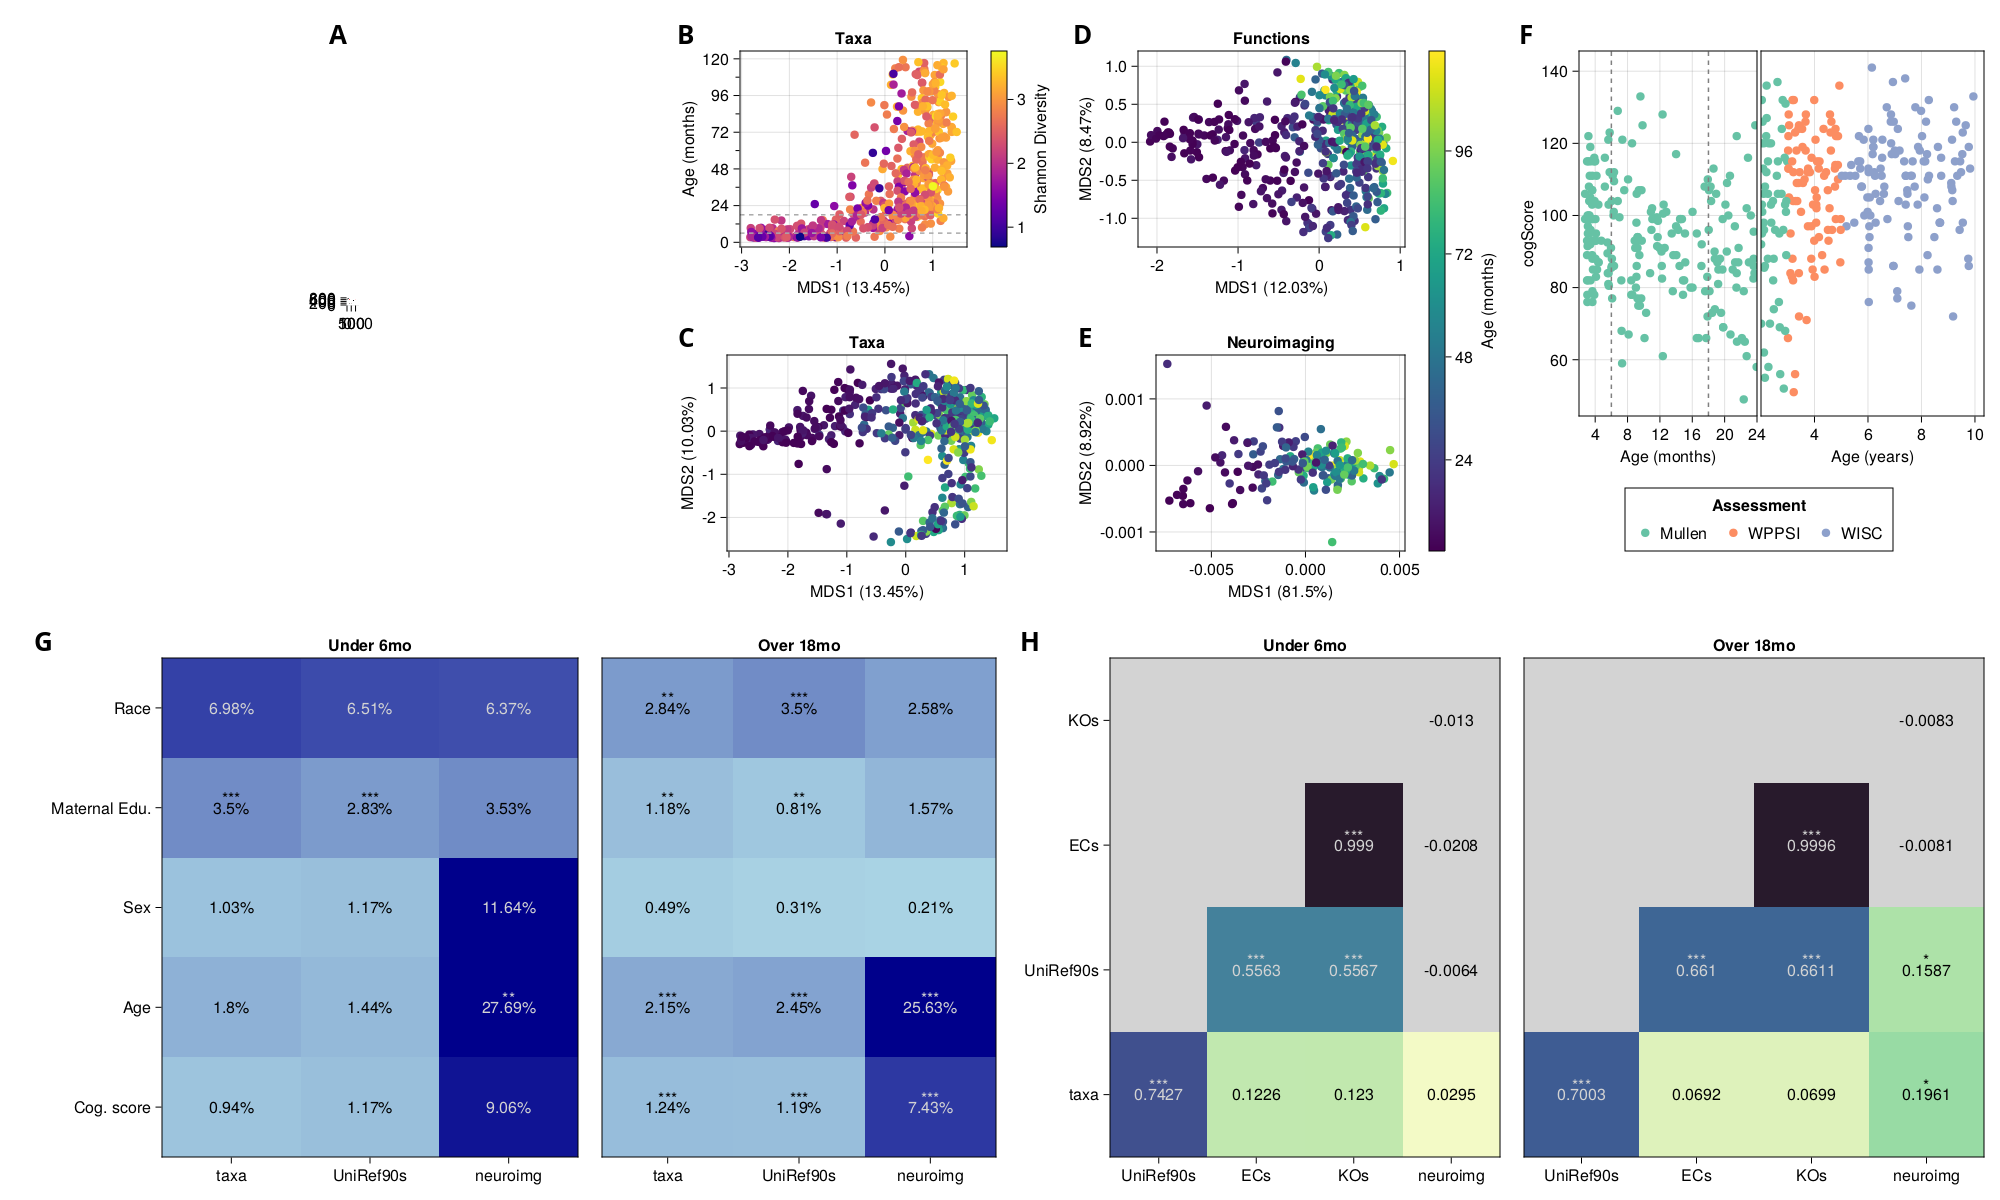
\includegraphics[width=0.9\textwidth]{assets/Figure1.png}
    \caption{
        Study design and overview. (\textbf{A}) Stool samples, cognitive assessments and
        neuroimaging were collected from participants in an accelerated
        longitudinal design. (\textbf{B}) Cognitive function scores are assessed by
        different instruments, but may be normalized to a common IQ-like scale.
        (\textbf{C-D}) Principal coordinates analysis using Bray-Curtis dissimilarity on
        taxonomic profiles demonstrates high beta diversity, with much of the
        first axis of variation explained by increasing age and alpha diversity.
        Differences in gene function profiles (\textbf{E}) and neuroimaging (PCA based on
        the Euclidean distance of brain region volumes) (\textbf{F}) are likewise
        dominated by changes as children age. (\textbf{G}) Permutation analysis of
        variance (PERMANOVA) of taxonomic profiles, functional profiles
        (annotated as UniRef90s) and neuroimaging, against the metadata of
        interest. Variations in taxonomic and functional profiles explain a
        modest but significant percent of the variation in cognitive development
        in children over 18 months of age. (\textbf{H}) Mantel testing of different
        microbial feature matrices, shows overlapping but distinct patterns of
        variation. Dotted lines in (B) and (C) show 6 and 18 months, which are
        used as cut-offs in some following models.
    }
    \label{fig:1}
\end{sidewaysfigure}


\begin{table}[!htb]
    \centering
    \begin{tabular}{|r|r|r|r|r|}
      \hline\hline
      \textbf{group} & \textbf{subgroup} & \textbf{all} & \textbf{under6mo} & \textbf{over18mo} \\\hline
      N subjects &  & 361 & 74 & 257 \\  \hline
    \multirow{3}{*}{Samples} & 1 & 262 (72.6\%) & 74 (100.0\%) & 203 (79.0\%) \\ \cline{2-5}
         & 2 & 72 (19.9\%) & 0 (0.0\%) & 46 (17.9\%) \\ \cline{2-5}
         & \textgreater 2 & 27 (7.5\%) & 0 (0.0\%) & 8 (3.1\%) \\ \hline
    \multirow{3}{*}{Age (months)} & min & 2.76 & 2.76 & 18.03 \\ \cline{2-5}
         & max & 119.3 & 6.0 & 119.3 \\ \cline{2-5}
         & median & 25.79 & 3.66 & 45.92 \\ \hline
    \multirow{2}{*}{Sex} & F & 163 (45.2\%) & 37 (50.0\%) & 114 (44.4\%) \\   \cline{2-5}
                         & M & 198 (54.8\%) & 37 (50.0\%) & 143 (55.6\%) \\  \hline
    \multirow{6}{*}{Race} & White & 252 (69.8\%) & 42 (56.8\%) & 191 (74.3\%) \\   \cline{2-5}
        & Black & 40 (11.1\%) & 16 (21.6\%) & 21 (8.2\%) \\ \cline{2-5}
        & Indiginous & 1 (0.3\%) & 0 (0.0\%) & 1 (0.4\%) \\ \cline{2-5}
        & Asian & 7 (1.9\%) & 1 (1.4\%) & 6 (2.3\%) \\ \cline{2-5}
        & Mixed & 48 (13.3\%) & 12 (16.2\%) & 29 (11.3\%) \\ \cline{2-5}
        & Other & 2 (0.6\%) & 1 (1.4\%) & 2 (0.8\%) \\ \hline
    \multirow{6}{*}{Maternal Ed.} & Junior high school & 1 (0.3\%) & 0 (0.0\%) & 1 (0.4\%) \\   \cline{2-5}
        & Some high school & 6 (1.7\%) & 3 (4.1\%) & 4 (1.6\%) \\ \cline{2-5}
        & High school grad & 37 (10.2\%) & 13 (17.6\%) & 16 (6.2\%) \\ \cline{2-5}
        & Some college & 95 (26.3\%) & 25 (33.8\%) & 57 (22.2\%) \\ \cline{2-5}
        & College grad & 90 (24.9\%) & 17 (23.0\%) & 69 (26.8\%) \\ \cline{2-5}
        & Grad/professional school & 123 (34.1\%) & 15 (20.3\%) & 104 (40.5\%) \\\hline\hline
    \end{tabular}
    \caption{\label{tab:demo}Subject demographics}
\end{table}

Several studies have demonstrated links between specific taxa and
measures of anxiety and depression
\cite{mayneris-perxachsMicrobiotaAlterationsProline2022,needhamGutderivedMetaboliteAlters2022},
cognitive flexibility in adults
\cite{magnussonRelationshipsDietrelatedChanges2015},
and atypical neural development
\cite{liuAlteredGutMicrobiota2019,wanUnderdevelopmentGutMicrobiota2021}.
We, therefore, set out to identify whether specific taxa
or gene functions were linked with normal cognitive development in
children. In order to assess whether variations in gut microbial taxa,
their genes, or their metabolism are linked with neurocognitive
development, we tested whether the beta diversity of microbial taxa and
gene functions, as well as variation in brain development as assessed by
neuroimaging, were associated with these contemporaneous measures of
cognitive function using permutation analysis of variance (PERMANOVA).
Due to the large ecological shift in the microbiome that occurs upon the
introduction of solid food, and a relatively wide range of ages when
infants are transitioned to solid food, we considered the pre-transition
(less than 6 months old) and post-transition (over 18 months old)
microbiomes separately. Even still, age was a major driver of variation
in gut microbiomes in children over 18 months old (Figure 1G). We also
found that overall variation in microbial species in children over 18
months old was associated with a small but significant variation in
cognitive function score (Figure 1G, R\textsuperscript{2} = 0.0124, q
\textless{} 0.001), as was variation in microbial gene functions
(R\textsuperscript{2} = 0.0119, q \textless{} 0.001). Variation in
microbial taxa and genes was not significantly associated with cognitive
function in children under 6 months, though this may be due to the low
taxonomic diversity, and broad lack of overlap between taxa in infants.
As expected, age was significantly associated with microbial beta
diversity (taxa R\textsuperscript{2} = 0.0215, and UniRef90s
R\textsuperscript{2} = 0.0245, q \textless{} 0.001), and very strongly
associated with neuroimaging profiles (R\textsuperscript{2} = 0.256, q
\textless{} 0.001).

Consistent with prior studies, different microbial measurement types
captured overlapping variation, with species profiles and gene function
profiles (annotated with clusters of 90\% similarity
\cite{suzekUniRefComprehensiveNonredundant2007}
), both generated from DNA sequencing data, being tightly coupled
(Figure 1H, p \textless{} 0.001). Interestingly, other functional
groupings (Enzyme commission level4 - ECs
\cite{bairochENZYMEDatabase20002000},
and
KEGG orthologues - KOs
\cite{kanehisaKEGGResourceDeciphering2004}
) overlapped only slightly with taxonomic profiles in both age
cohorts, despite being derived from UniRef90 labels. In children over 18
months, some variation (15.9\%, p \textless{} 0.01) in neuroimaging
overlapped with microbial measures, though this may be due to the
residual variation due to age in both measures.

\subsubsection*{Microbial species and neuroactive genes are associated with cognitive performance}

To assess whether individual microbial species were associated with
cognitive function, we fit multivariable linear regression
\cite{mallickMultivariableAssociationDiscovery2021}
to the relative abundance of each species that had at least 15\%
prevalence in a given age group (Figure 2A, N = 92 for 0--120 months, N
= 46 for 0--6 months, N = 97 for 18--120 months). Only \emph{Blautia wexlerae}
was significantly associated (q value = 0.14, $\beta$ = 0.0015) with
cognitive function in children under 6 months old after adjusting for
age and maternal education (Figure 2B). \emph{B. wexlerae} was
previously shown to be depleted in children with diabetes
\cite{benitez-paezDepletionBlautiaSpecies2020},
and that oral administration of \emph{B. wexlerae} partially
ameliorated weight gain and inflammation from a high-fat diet in a mouse
model of T2D
\cite{hosomiOralAdministrationBlautia2022,liuBlautiaNewFunctional2021}.
In children over 18 months of age,
several microbial species were significantly enriched (q-value
\textless{} 0.20) in children with higher cognitive function scores,
including \emph{Gordonibacter pamelaeae}, which produces the
neuroprotective metabolite urolithin
\cite{gongUrolithinAlleviatesBloodbrain2022,selmaDescriptionUrolithinProduction2014},
\emph{Asaccharobacter celatus} and
\emph{Adelcreutzia equolifaciens}, which produce phytoestrogen-derived
equol
\cite{maruoAdlercreutziaEquolifaciensGen2008,thawornkunoBiotransformationDaidzeinEquol2009},
and the SCFA-producing probiotic
species such as \emph{Eubacterium eligens} and \emph{Faecalibacterium
prausnitzii}
\cite{ghoshMediterraneanDietIntervention2020}
(Figure 2B).

\begin{sidewaysfigure}[!htb]
    \centering
    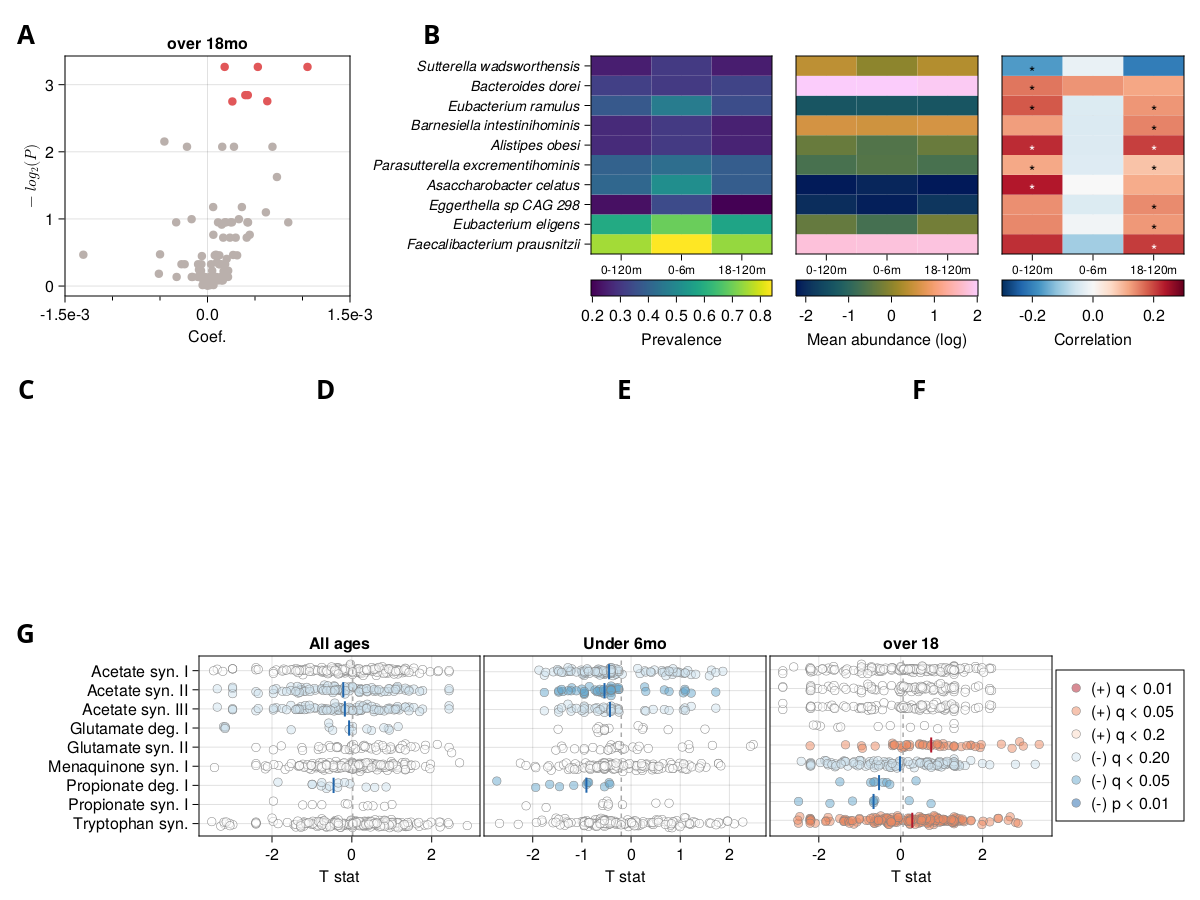
\includegraphics[width=\textwidth]{assets/Figure2.png}
    \caption{
        Taxa and gene functional groups are associated with cognitive function.
        (\textbf{A}) Volcano plot of multivariable linear model results showing the
        relationship between individual taxa and cognitive function score in
        children over 18 months of age, controlling for age, maternal education,
        and sequencing depth. Taxa that were significant after FDR correction (q
        \textless{} 0.2) are colored red. (\textbf{B}) For taxa that were significantly
        associated with cognitive function, heatmaps of prevalence, mean
        relative abundance, and correlation with cognitive function in different
        age groups. (\textbf{C-F}) Enrichment plots for selected neuroactive gene sets
        used in feature set enrichment analysis (FSEA). (\textbf{G}) summary of FSEA
        results across all samples (left) as well as in the under 6 months
        (middle) and over 18 months (right) subsets, colored based on the
        significance of the association. Markers indicate the individual
        correlation of genes within a gene set, and vertical bars represent the
        median correlation of that gene set.
    }
    \label{fig:2}
\end{sidewaysfigure}

Given that different microbial species might occupy the same metabolic
niche in different individuals, we hypothesized that microbial genes
grouped by functional activity would be associated with cognition. To
test this, we performed feature set enrichment analysis (FSEA) on groups
of genes with neuroactive potential
\cite{valles-colomerNeuroactivePotentialHuman2019}
and concurrent cognitive function score (Table 2, Figure 2C-G) and found that
several metabolic pathways were significantly enriched or depleted in
children with higher cognitive function scores. This was true both when
considering all age groups together, though the enrichment of most
pathways was more pronounced in children under 6 months or over 18
months. For example, genes for degrading the 3-carbon SCFA propionate
were significantly depleted in children with higher cognitive function
scores across all age groups tested (Table 2; propionate degradation I,
under 6 months, enrichment score (E.S.) = -0.542, corrected p-value (q)
= 0.020; over 18 months, E.S. = -0.674, q = 0.041). Interestingly, genes
for propionate synthesis were also significantly depleted in higher
scoring children over 18 months (E.S. -0.676, q = 0.023), as were genes
for synthesizing the 2 carbon SCFA acetate in children under 6 months
old (acetate synthesis I, E.S. = -0.194, q = 0.153; acetate synthesis
II, E.S. = -0.342, q = 0.020; acetate synthesis III, E.S. = -0.31, q = 0.052).
SCFAs are produced by anaerobic fermentation of dietary fiber
and have been linked with immune system regulation as well as directly
with brain function \cite{dalileRoleShortchainFatty2019}.


Synthesis of menaquinone (vitamin K) was also negatively associated with
cognitive function score in older children (menaquinone synthesis I,
E.S. = -0.170, q = 0.0183). Menaquinone has several isoforms, one of
which, MK-4, has been found to be decreased in children diagnosed with ASD
\cite{dongCorrelationSerumConcentrations2021}
and is potentially neuroprotective in both rodents and humans
\cite{elkattawyVitaminK2Menaquinone72022}.
In children over 18 months old,
genes for the synthesis of the amino acids
glutamate and tryptophan were significantly enriched in children with
higher cognitive function scores (Glutamate synthesis I, E.S. = 0.242, q
= 0.047; Tryptophan synthesis, E.S. = 0.119, q = 0.041). Glutamate is a
critical neurotransmitter controlling neuronal excitatory/inhibitory
signaling along with gamma-aminobutyric acid (GABA), and their balance
in the brain controls neural plasticity and learning, particularly in
the developing brain
\cite{cohenkadoshLinkingGABAGlutamate2015,palomo-buitragoGlutamateInteractionsObesity2019}.
Tryptophan metabolism, including
microbial metabolism of tryptophan, has previously been linked with
autism in children
\cite{hoshinoBloodSerotoninFree1984,xiaoFecalMicrobiomeTransplantation2021}.
Taken together, these results suggest that
microbial metabolic activity, particularly the metabolism (synthesis and
degradation) of neuroactive compounds may have effects on cognitive
development.


\begin{table}[!h]
    \begin{center}
    \begin{tabular}{|r|r|r|r|r|r|r|}
      \hline\hline
      \textbf{Age group} & \multicolumn{2}{c}{\textbf{00to120}} & \multicolumn{2}{c}{\textbf{00to06}} & \multicolumn{2}{c}{\textbf{18to120}} \\ \hline
      \texttt{geneset} & \texttt{E.S.} & \texttt{q value} & \texttt{E.S.} & \texttt{q value} & \texttt{E.S.} & \texttt{q value} \\\hline
      Acetate syn. I & -0.122 & 0.555 & -0.194 & \color{red}{\textbf{0.153}} & 0.127 & 0.602 \\
      Acetate syn. II & -0.22 & \color{red}{\textbf{0.066}} & -0.342 & \color{red}{\textbf{0.02}} & -0.095 & 0.92 \\
      Acetate syn. III & -0.21 & \color{red}{\textbf{0.086}} & -0.31 & \color{red}{\textbf{0.052}} & -0.086 & 0.92 \\
      Glutamate deg. I & -0.404 & \color{red}{\textbf{0.18}} & -0.284 & 0.816 & -0.249 & 0.602 \\
      Glutamate syn. II & 0.095 & 0.602 & -0.134 & 0.98 & 0.242 & \color{blue}{\textbf{0.047}} \\
      Menaquinone syn. I & -0.085 & 0.563 & -0.083 & 0.816 & -0.17 & \color{red}{\textbf{0.182}} \\
      Propionate deg. I & -0.461 & \color{red}{\textbf{0.13}} & -0.542 & \color{red}{\textbf{0.02}} & -0.674 & \color{red}{\textbf{0.041}} \\
      Propionate syn. I & -0.334 & 0.555 & -0.32 & 0.571 & -0.676 & \color{red}{\textbf{0.023}} \\
      Tryptophan syn. & 0.057 & 0.974 & -0.072 & 0.816 & 0.119 & \color{blue}{\textbf{0.041}} \\\hline\hline
    \end{tabular}
    \caption{\label{tab:fsea}Feature set enrichment analysis on neuroactive microbial gene sets}
    \end{center}
\end{table}


\subsubsection*{Gut microbial taxonomic and functional profiles predict cognitive function}

FSEA relies on understanding functional relationships between individual
genes. However, because the relationships between individual taxa are
still largely unknown, we turned to Random Forest (RF) models, an
unsupervised non-parametric machine learning (ML) method that enables
the identification of underlying patterns in large numbers of individual
features (here, microbial species). Previous studies have reported
successful use of RFs for processing highly-dimensional and sparse data
from the domain of genomics
\cite{amaratungaEnrichedRandomForests2008,brieucPracticalIntroductionRandom2018,chenRandomForestsGenomic2012,franzosaGutMicrobiomeStructure2019,stephanRandomForestApproach2015},
along with other works where it was used
to predict cognitive conditions related to Alzheimer's disease in
different scenarios
\cite{ardekaniPredictionIncipientAlzheimer2017,velazquezRandomForestModel2021}.
Additionally, given the sequential
nature of variable consideration in each tree, RFs are naturally able to
work out complex input feature interactions, such as those present in a
microbiome-wide study, without the necessity to explicitly compute
interaction terms.

\begin{sidewaysfigure}[!htb]
    \centering
    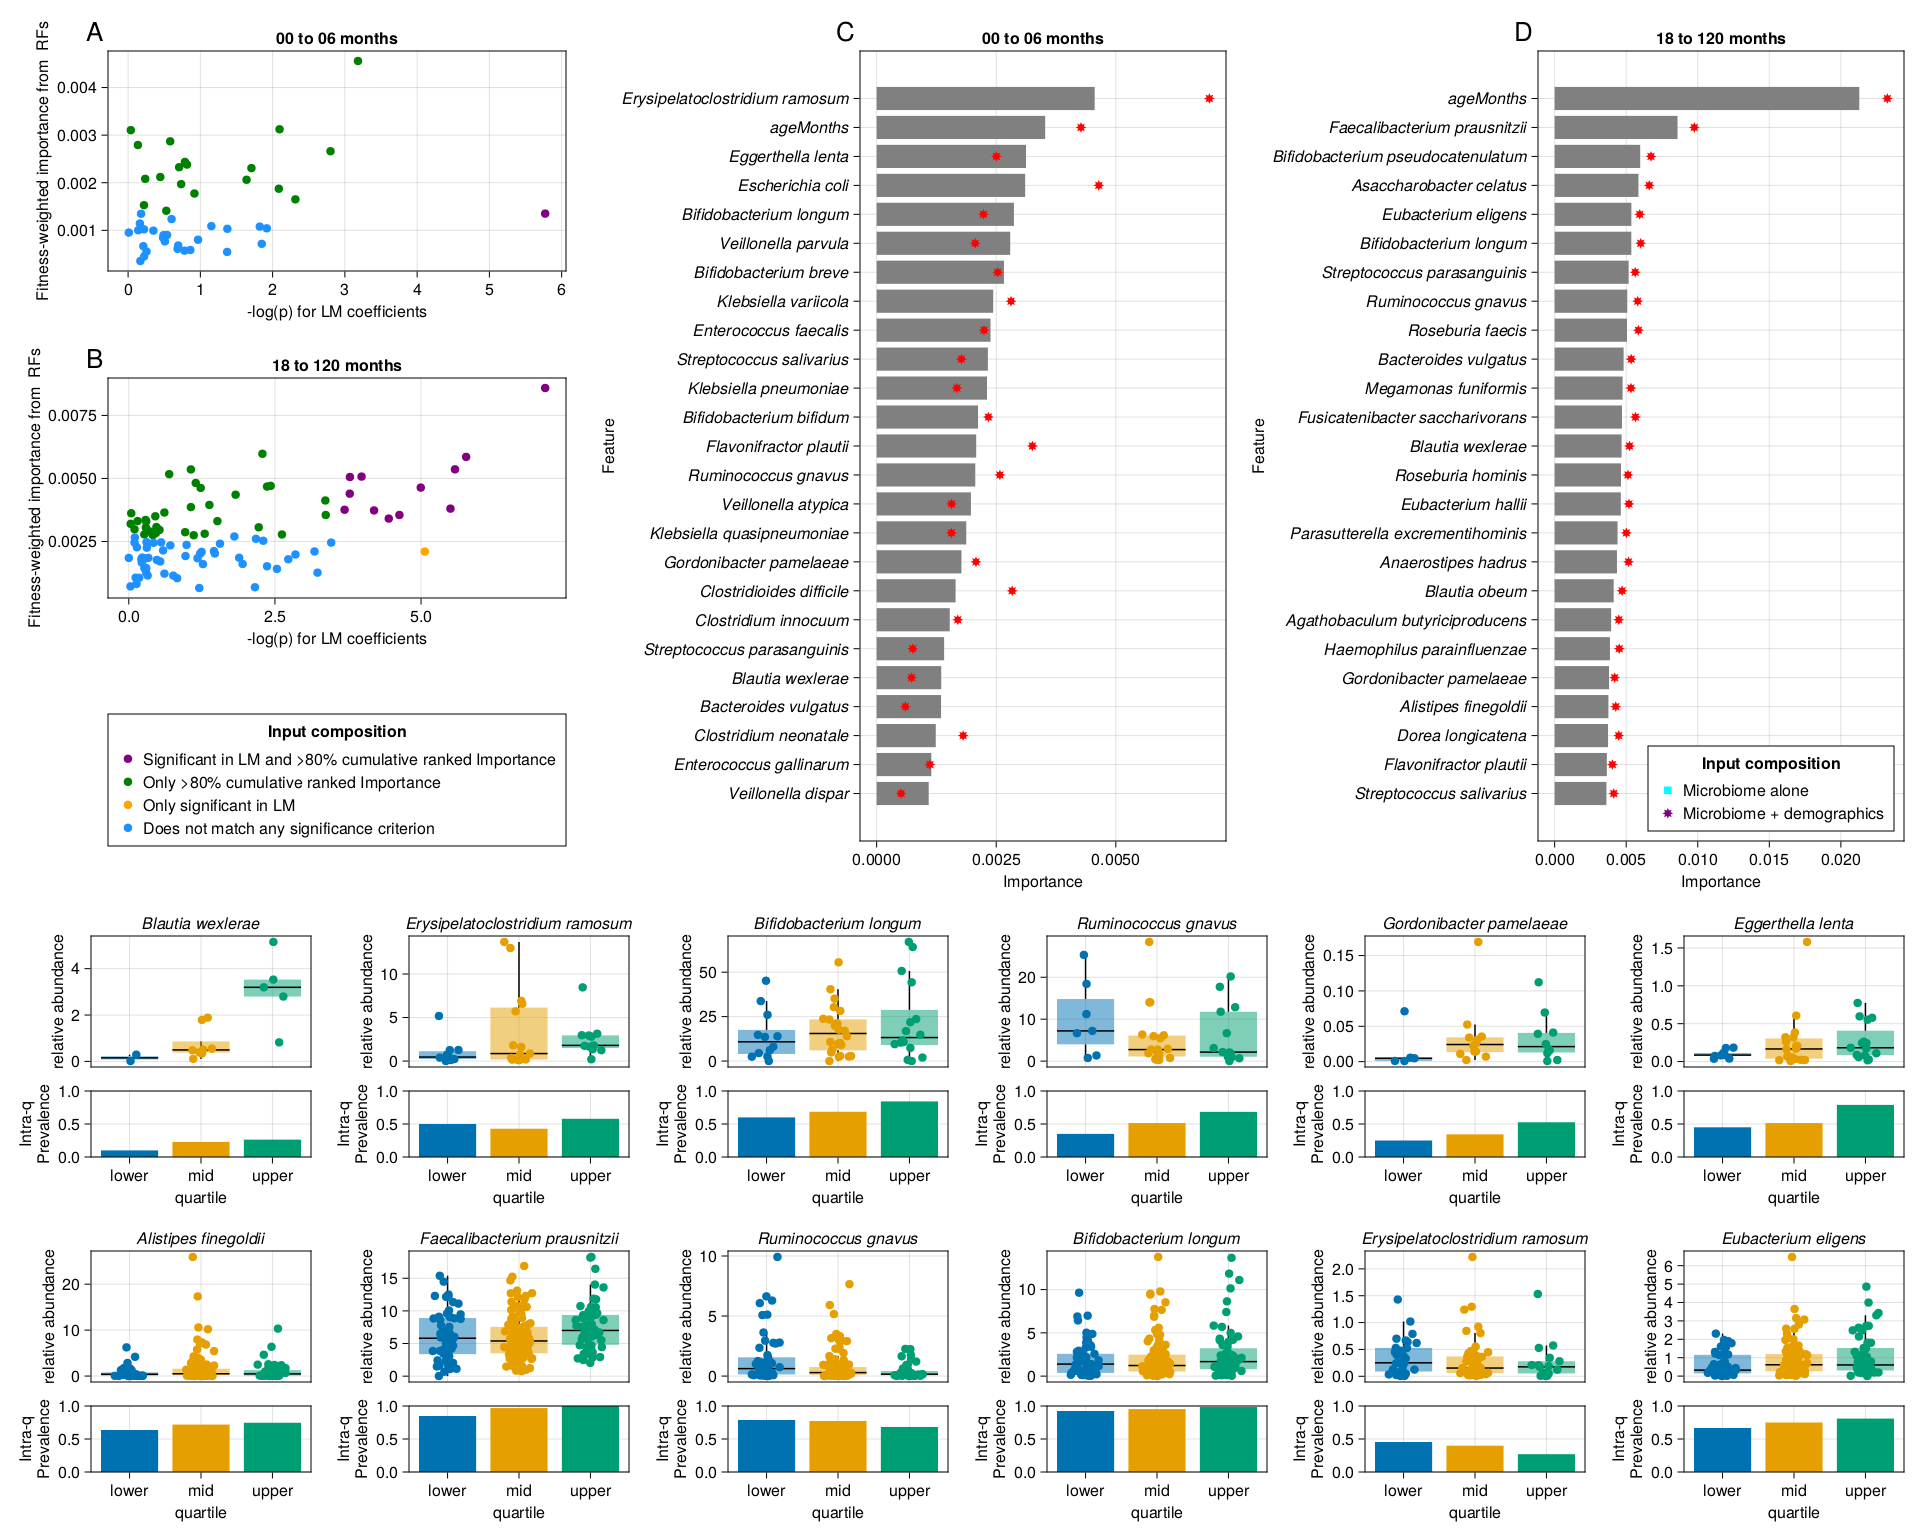
\includegraphics[width=\textwidth]{assets/Figure3.png}
    \caption{
        Random forest models predict concurrently measured cognitive function.
        Comparison of RF predictor importance versus linear models for children
        between birth and 6 months old (\textbf{A}), and for those older than 18 months
        (\textbf{B}). Colors represent whether the species belong to the group of
        top-important features that account for 80\% of the cumulative
        importance on the RF model, if that species was significant (q
        \textless{} 0.2) in linear models, both, or neither. Ranked feature
        importance for taxa in RF models for children between birth and 6 months
        old (\textbf{C}), and for those older than 18 months (\textbf{D}). Taxa that are important
        for RF models both for children under 6 months and for those over 18
        months (\textbf{E}), only for children under 6 months (\textbf{F}), and only for children
        over 18 months (\textbf{G})
    }
    \label{fig:3}
\end{sidewaysfigure}


Given that gut microbial profiles, as well as neurocognitive
development, may partially reflect socioeconomic and demographic
factors, we assessed the performance of RF regressors where maternal
education (a proxy of socioeconomic status (SES)), sex, and age were
included as possible predictors, either alone or in combination with
microbial taxonomic profiles (Table 3).

\textbf{Table 3. Benchmark metrics for the cognitive assessment score
prediction models. Confidence intervals are calculated from the
distribution of metrics from repeated CV at a confidence level of 95\%}

\begin{table}
    \begin{tabular}{rrrrr}
      \hline\hline
      \textbf{Subject Ages (months)} & \textbf{Microbial feature} & \textbf{Demo.} & \textbf{Test set correlation (± C.I.)} & \textbf{Test set Root-mean-square error (± C.I.)} \\\hline
      0 to 6 & - & + & 13.01 ± 0.05 & -0.14 ± 0.01 \\
      0 to 6 & taxa & - & 12.66 ± 0.05 & -0.1 ± 0.01 \\
      0 to 6 & taxa & + & 12.7 ± 0.05 & -0.12 ± 0.01 \\
      0 to 6 & genes & - & 12.56 ± 0.05 & -0.01 ± 0.01 \\
      0 to 6 & genes & + & 12.56 ± 0.05 & -0.02 ± 0.01 \\
      18 to 120 & - & + & 16.27 ± 0.04 & 0.506 ± 0.003 \\
      18 to 120 & taxa & - & 17.66 ± 0.04 & 0.363 ± 0.003 \\
      18 to 120 & taxa & + & 17.29 ± 0.04 & 0.429 ± 0.003 \\
      18 to 120 & genes & - & 18.01 ± 0.04 & 0.303 ± 0.003 \\
      18 to 120 & genes & + & 17.86 ± 0.04 & 0.333 ± 0.004 \\\hline\hline
    \end{tabular}
\end{table}

As with linear models, RF models for children under 6 months old were
less generalizable (mean test-set correlation -0.13, mean RMSE 12.70),
but RFs were consistently able to learn the relationship between taxa
and cognitive function scores in children over 18 months of age (mean
test-set correlation 0.429, mean RMSE 17.29). For both age groups,
species that were important in RF overlapped with those that were
significant when testing the relationship with linear models (Figure
3A-B, Supplementary Table XXA-B), though there were substantial
differences. For children under 6 months, only \emph{B. wexlerae} was
significantly associated with cognitive function in linear models, but
was ranked 20th in importance for RF models. The importance metric
employed (MDI) is a measure of how well the variable differentiates
(splits) sets of samples by creating subgroups that reduce the
intra-group deviations, while also accounting for the amount of samples
affected by a split. All taxa significantly associated with cognitive
function score in children over 18 months using LMs belong to the
top-ranking group responsible for 80\% of the total relative importance,
except for \emph{Eubacterium ramulus} (Table 3, Figure 3A).

Interestingly, several taxa highly ranked in importance in both age
groups, including several that were significant in LMs for children over
18 months old, including \emph{R. gnavus} (0--6 months, rank = 13;
18--120 months, rank = 7) and \emph{G. pamelaeae} (0--6 months, rank =
16; 18--120 months, rank = 20), while others such as \emph{Allistipes
finegoldii} were age-group specific. Several taxa important in RF models
were not statistically significant when using linear models after
multiple hypothesis correction. However, these taxa had small nominal
p-values. For example, \emph{Erysipelatoclostridium ramosum} was the
most important feature in RF models for children under 6 months old and
had an LM p-value of 0.04. Subject age was consistently ranked highly in
feature importance, which could indicate that decision branches based on
microbial taxa have increased purity when considering the subject's age
or that age itself is a useful predictor.

\subsubsection*{Gut microbial taxonomic profiles predict brain structure differences}

If there are causal effects of microbial metabolism on cognitive
function, they might be reflected in changes in neuroanatomy. We again
employed a Random Forest modeling approach to associate gut taxonomic
profiles with individual brain regions identified in MRI scans,
normalized to total brain volume. Some brain regions were more readily
predicted by RF models trained on microbial taxa (Table 4, Supplementary
Table XX), in particular those that were highly correlated with age.
These included the L/R lingual gyrus (mean RF correlations, Left =
0.421, Right = 0.434; relative age importances, Left = 7.5\%, Right =
8.3\%) and the L/R pericalcarine cortex (mean RF correlations, Left =
0.200, Right = 0.273; relative age importances, Left = 3.7\%, Right =
6.3\%). In many cases, however, age was not an important variable in
high-performing models, such as that for the left accumbens area (mean
RF correlations = 0.288; relative age importances = 1.2\%).

\textbf{Table 4. Summary statistics for the neuroanatomy prediction benchmarks}

\begin{table}
    \begin{tabular}{rrr}
      \hline\hline
      \textbf{Statistic} & \textbf{Mean absolute proportional error (MAPE)} & \textbf{Correlation coefficient (R)} \\\hline
      Mean & 0.073 & 0.137 \\
      Standard deviation & 0.028 & 0.137 \\
      Maximum & 0.206 & 0.605 \\
      75th percentile & 0.082 & 0.195 \\
      50th percentile & 0.067 & 0.134 \\
      25th percentile & 0.057 & 0.062 \\
      Minimum & 0.035 & -0.147 \\\hline\hline
    \end{tabular}
\end{table}

We also observed that many brain regions had high accordance across the
left and right hemispheres in terms of both model performance and
microbial feature importance. In contrast, other regions had substantial
differences between the hemispheres. For example, the left accumbens
area, which plays an important role in reward circuits
\cite{ernstAmygdalaNucleusAccumbens2005,yauNucleusAccumbensResponse2012},
has one of the highest test-set correlations of our
brain region models (R = 0.288), as compared to the right accumbens
models which could not adequately generalize, and had a negative mean
test-set correlation (R = -0.041). Most healthy individuals have a
rightward asymmetry in the nucleus accumbens, and reduced asymmetry has
been linked to substance use disorder in young adults
\cite{caoMappingCorticalSubcortical2021}.

Feature importance for models of the left accumbens area were dominated
by three species of \emph{Bacteroides}, \emph{B. vulgatus} (3.4\%
relative importance), \emph{B. ovatus} (3.7\% relative importance), and
\emph{B. uniformis} (3.0\% relative importance).. The accumbens area is
associated with reward control, and in individuals diagnosed with ADHD,
it has been shown to have a divergent neuromorphology
\cite{hoogmanSubcorticalBrainVolume2017}.
Independently, \emph{B. ovatus}, \emph{B. uniformis} and
\emph{B. vulgatus} have been linked to ADHD
\cite{wangGutMicrobiotaDietary2020}.

In fact, there are studies showing that alterations on the striatal
dopamine transporters can cause effects resembling hyperactivity and
attention deficit
\cite{yaelDisinhibitionNucleusAccumbens2019},
and that \emph{B. uniformis} is gut-microbial modulator of the brain
dopamine transporter
\cite{hartstraInfusionDonorFeces2020}.


Many of the taxa identified included taxa also identified in LMs and RF
models of cognitive function. Interesting to note, while RF models for
multiple brain regions had many important microbial taxa, others were
dominated by a small number of taxa. In general, for all segments, a
consistent number of species between 14 and 22 (median = 20) was
responsible for one third of the fitness-weighted cumulative importance
(see Methods), regardless of the model benchmarks. We proceeded to
select a subset of the most important taxa (averaged over all segments)
and the segments whose importance was more heavily loaded to further
analyze the multiple relationships unveiled by the RF models
(Figure 4 A and B)

\begin{sidewaysfigure}[!htb]
    \centering
    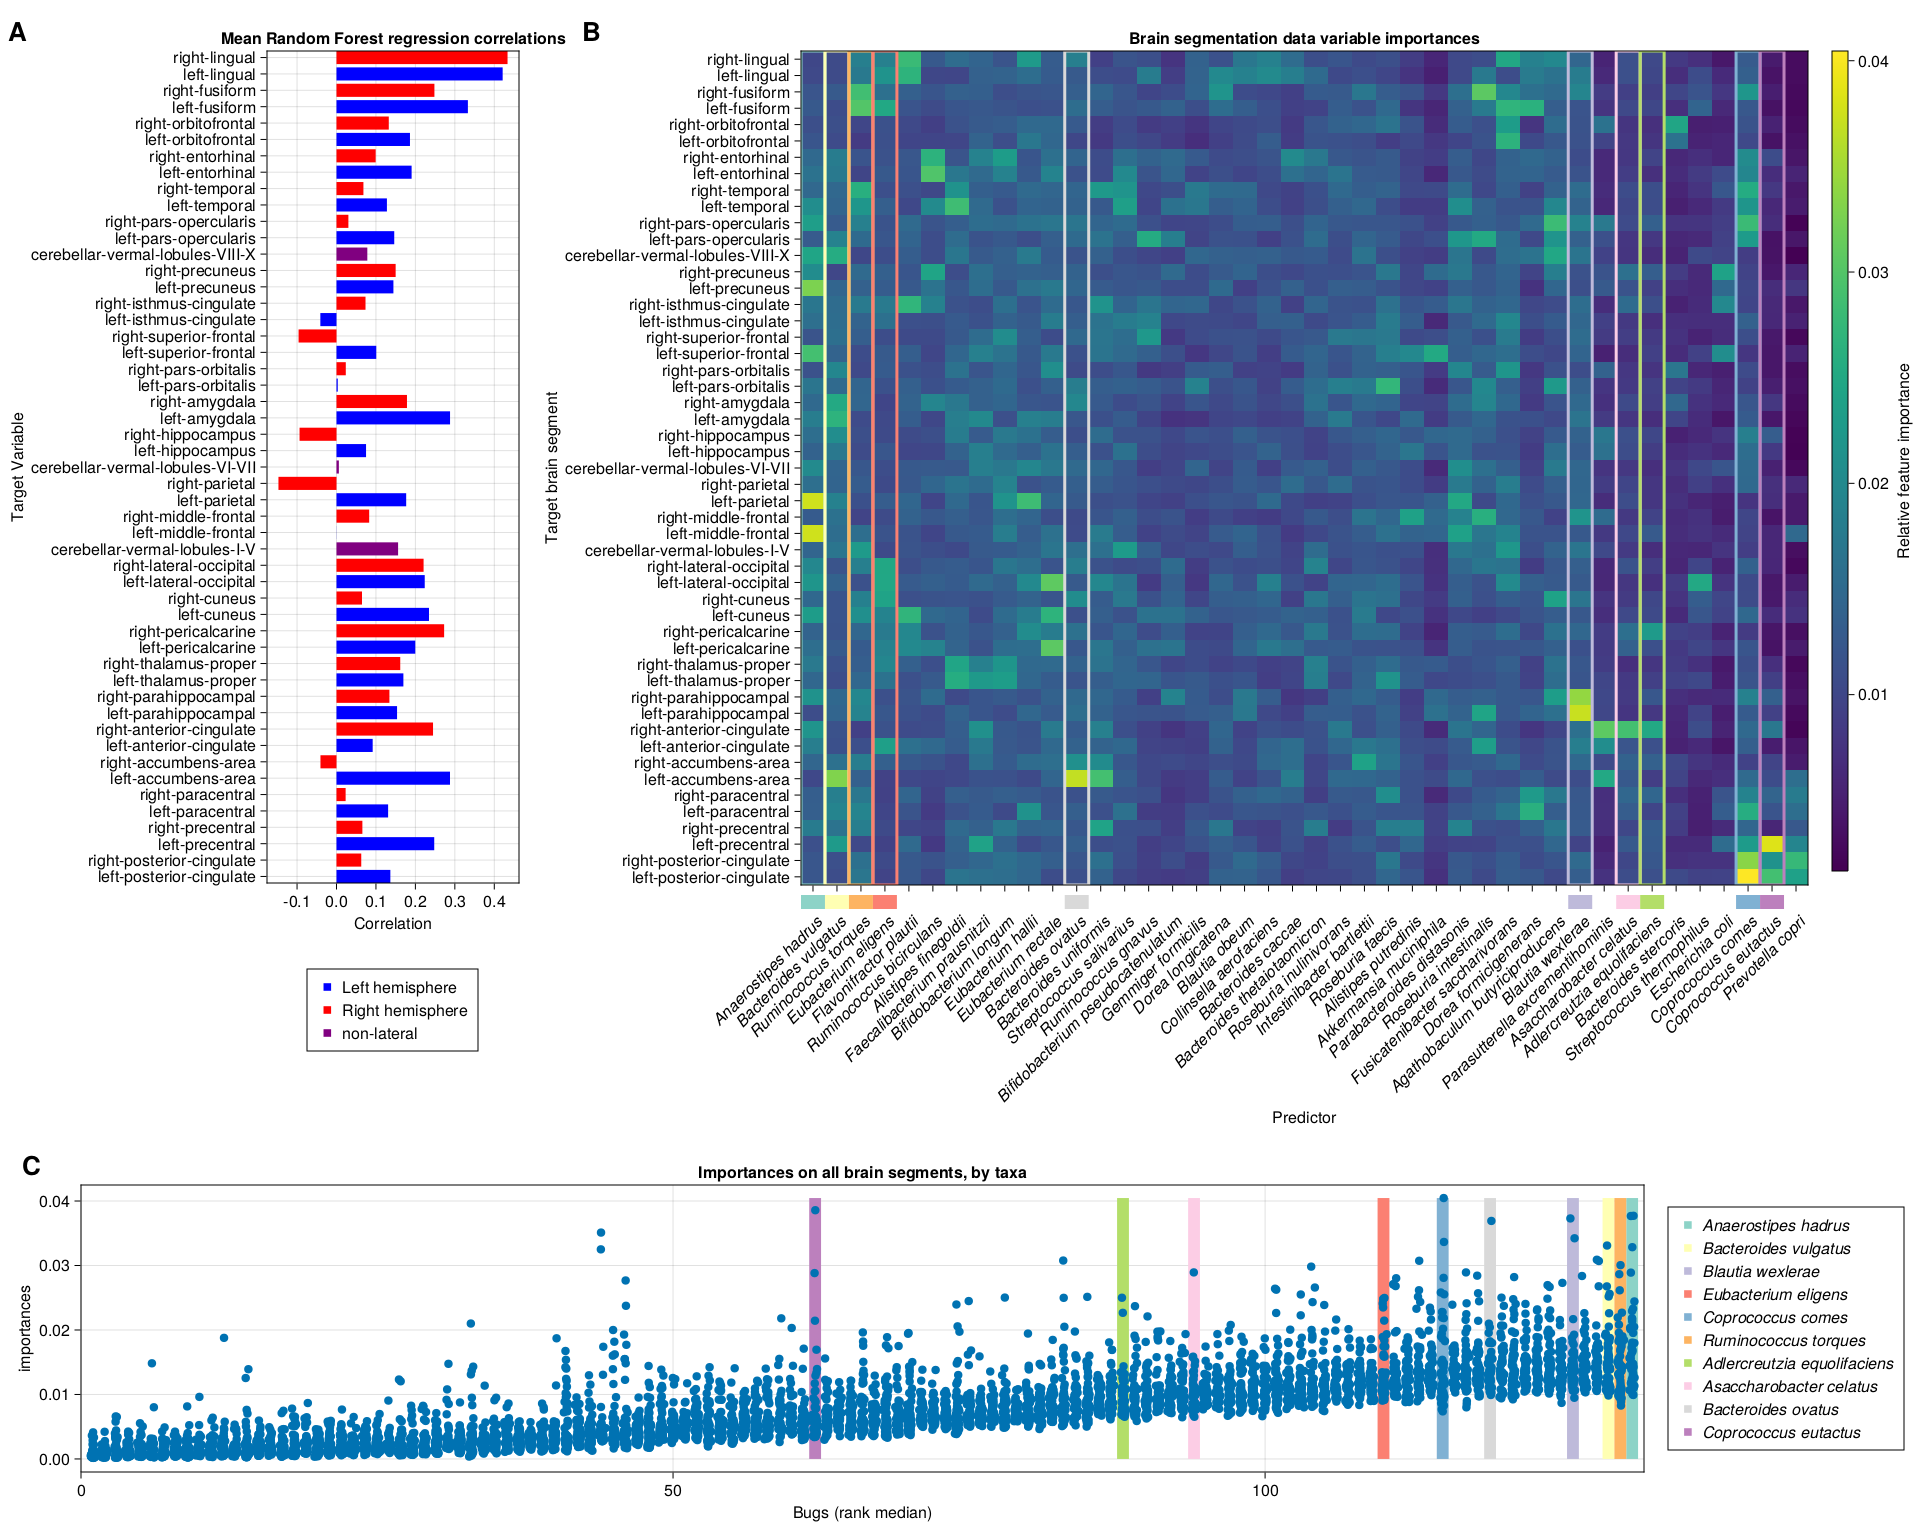
\includegraphics[width=\textwidth]{assets/Figure4.png}
    \caption{
        Microbial feature importance in predicting brain volumes in children over 18 months of age.
        (\textbf{A}) Average test-set correlations for prediction of MRI segmentation
        data from microbiome and demographics on select segments after repeated
        cross validation. (\textbf{B}) Heatmap of average individual relative taxa
        importances on each brain segment. Importances are reported as
        proportions relative to the sum of importances for each model - since
        every model is trained with 132 features, and even distribution of
        importance would be 0.75\% for each feature. Segments and taxa ordered
        by HCA on a select list of species with high ranks on average importances,
        and their respective highest-load segments (\textbf{C}).
    }
    \label{fig:4}
\end{sidewaysfigure}


Our analysis revealed two major patterns of importance distribution from
taxa over the brain segments; some species portrayed high contributions
to multiple different segments, while others contributed modestly to
just one or two brain segments. Notable cases of the first pattern
included seven species - \emph{Anaerostipes hadrus}, \emph{Bacteroides
vulgatus}, \emph{Fusicatenibacter saccharivorans}, \emph{Ruminococcus
torques}, \emph{Eubacterium rectale}, \emph{Coprococcus comes} and
\emph{Blautia wexlerae} - that combined, account for approximately one
third of the cumulative relative importances, computed after subsetting
on the taxa of interest (Figure 4C).

Among these, the most important variable is \emph{Anaerostipes hadrus},
which is a butyrate-producing anaerobe that has been positively
associated with cognitive function
\cite{kantGenomeSequenceButyrateProducing2015,liCorrelationsGutMicrobiota2022}.
Its importance is, however, heavily loaded on the volume
of entire major lobes (frontal, parietal), which cannot be readily
correlated to specific cognitive functions. After accounting for the
major lobes, it is found to be highly important on the prediction of the
cerebellar vermal lobules VIII-X, pars opercularis, cuneus and
precuneus, and anterior-cingulate (Figure 4B).

To better understand this relationship, we performed hierarchical
cluster analysis, which revealed a well defined cluster of species with
high importance loadings on close segments of the lower temporal and
close occipital lobe, to which \emph{A. hadrus} belongs. The other
species on this cluster are \emph{B. wexlerae}, \emph{R. torques},
\emph{R. intestinalis, R. bicirculans} and \emph{F. saccahrivorans}, who
contribute heavily to the entorhinal, fusiform, lingual and
parahippocampal segments.

This group of taxa and their related segments drew our attention because
they contained \emph{B. wexlerae}, a highlight from the cognitive
assessment results. Previous works exploring Parkinson Disease patients
found out that issues in the cognitive task of confrontation naming were
positively correlated with thinning in the fusiform gyrus and
parahippocampal gyrus
\cite{pagonabarragaPatternRegionalCortical2013}.
Additionally, the left and right parahippocampal, where \emph{B.
wexlerae} had the highest importance in both models, are important in
visual/spatial processing and memory
\cite{aminoffRoleParahippocampalCortex2013}.
\emph{B. wexlerae} can also produce acetylcholine in the gut
\cite{hosomiOralAdministrationBlautia2022},
and this molecule plays an important role in modulating memory
function
\cite{haamCholinergicModulationHippocampal2017}.


Another notable importance cluster contains taxa associated with the
basal forebrain, especially the cingulate and the accumbens. This
cluster contains the previously-discussed \emph{B. ovatus} and \emph{B.
uniformis,} but also \emph{Alistipes finegoldii and Streptococcus
salivaris.} Reduction in the nucleus accumbens has been associated with
depression symptoms
\cite{wackerRoleNucleusAccumbens2009},
and increased levels of the \emph{Alistipes} genus have been
observed in patients with depressive disorder
\cite{jiangAlteredFecalMicrobiota2015}.
While these reports are important, simultaneously probing of the gut
metagenome and brain structure relationship is novel.

Both \emph{A. equolofaciens} and \emph{A. celatus,} two closely-related
equol-producing species, are examples of the second contribution
pattern, and had high importance in predicting the relative volume of
the right anterior cingulate (respectively, 3.0\% and 2.6\% relative
importances), which has been linked to social cognition and reward-based
decision making
\cite{appsAnteriorCingulateGyrus2016,boesRightAnteriorCingulate2008,bushDorsalAnteriorCingulate2002}.
Equol has a strong estrogenic effect
\cite{setchellSEquolPotentLigand2005},
and in anterior cingulate, estrogen, has been shown to regulate
pain-related aversion
\cite{xiaoEstrogenAnteriorCingulate2013}.

Another example of this pattern is \emph{R. gnavus,} which was the only
species with significant negative association with cognitive function.
It is heavily associated with the left pars opercularis (2.7\% relative
importance), a relationship that may be explained by the emerging
understanding that this species is increased in individuals with insulin
resistance and obesity \cite{leyHumanGutMicrobes2006},
conditions that are known to produce structural abnormalities in the brain
\cite{opelBrainStructuralAbnormalities2021}.
Finally, \emph{Coprococcus comes} displays an importance
distribution that splits almost evenly among the two previously reported
clusters. Its loading on the prediction of the left posterior cingulate
is the highest for a microbe in RF models (4.0\% relative importance)
(only age had higher relative importance in any model), while also being
one of the most important predictors for neighboring areas of the
posterior cingulate such as the pars opercularis (relative importances,
Left = 2.3\%, Right = 2.8\%), along with upper regions like the left
precentral (2.3\% relative importance) and paracentral lobes (relative
importances, Left = 2.6\%, Right = 1.8\%).

\section*{Discussion}

The relationship between the gut microbiome and brain function via the
gut-microbiome-brain axis has gained increasing acceptance largely as a
result of human epidemiological studies investigating atypical
neurocognition (eg anxiety and depression, neurodegeneration, attention
deficit / hyperactivity disorder, and autism) and mechanistic studies in
animal models. The results from these studies point to the possibility
that gut microbes and their metabolism may be causally implicated in
cognitive development, but this study is the first to our knowledge that
directly investigates microbial species and their genes in relation to
typical development in young children. Understanding the gut-brain-axis
in early life is particularly important, since differences or
interventions in early life can have outsized and longer-term
consequences than those at later ages. Further, even in the absence of
causal impacts of microbial metabolism, identifying risk factors that
could point to other early interventions would also have value.

The use of shotgun metagenomic sequencing enabled us to get
species-level resolution of microbial taxa. A previous study of
cognition in 3 year old subjects used 16S rRNA gene amplicon sequencing,
and showed that genera from the Lachnospiraceae family as well as
unclassified Clostridiales (now Eubacteriales) were associated with
higher scores on the Ages and Stages Questionnaire
\cite{sordilloAssociationInfantGut2019}.
However, each of these clades encompass dozens of genera with
diverse functions, each of which may have different effects. Indeed,
several of the taxa that were positively associated with cognitive
function in this study, including \emph{B. wexlerae}, the only species
identified by linear models in children under 6 months, \emph{D.
longicatena}, \emph{R. faecis}, and \emph{A. finegoldii} are
Clostridiales, as is \emph{R. gnavus}, which we found was negatively
associated with cognitive function (Figure 2A-B). This kind of
species-level resolution is typically not possible with amplicon
sequencing.

We identified several species in the family Eggerthelaceae that were
associated with cognitive function, including \emph{Gordonibacter
pamelaeae, Aldercreutzia equolofaciens, Asaccharobacter celatus}
(formerly regarded a subspecies of \emph{A. equolofaciens}
\cite{takahashiCompleteGenomeSequence2021}),
and \emph{Eggerthella lenta}. Many members of this family are
known in part due to unique metabolic activities. For example, \emph{A.
equolofaciens} produces the nonsteroidal estrogen equol from isoflaven
found in soybeans
\cite{wangEnantioselectiveSynthesisSEquol2005},
and \emph{G. pamelaeae} can metabolize the polyphenol ellagic acid
(found in pomegranates and some berries) into urolithin, which has been
shown in some studies to have a neuroprotective effect
\cite{gongUrolithinAlleviatesBloodbrain2022,selmaDescriptionUrolithinProduction2014}.
\emph{E. lenta} has been extensively studied for
its ability to metabolize drug compounds such as the plant-derived heart
medication digoxin
\cite{haiserPredictingManipulatingCardiac2013}.
The metabolic versatility of this clade, and the large number of
species that are associated with cognition make these microbes prime
targets for further mechanistic studies.

In addition to improved species-level resolution, shotgun metagenomic
sequencing also enables gene-functional insight. We showed here that
genes for the metabolism of SCFAs, both their degradation and synthesis,
are associated with cognitive function scores. However, while the
differential abundance of genes for the metabolism of neuroactive
compounds like these is suggestive, it is difficult to reason about the
relationship between levels of these genes and the gut concentrations of
the molecules their product enzymes act on. For example, while it might
be intuitive to reason that increased levels of menaquinone synthesis
genes is indicative of increased menaquinone, it could be the case that
menaquinone deficiency selects for microbes that can synthesize it. For
the same reason, increased propionate degradation genes may
counterintuitively be indicative of high levels of propionate in the gut
lumen, since high propionate would select for microbes that can
metabolize it. For this reason, future studies coupling shotgun
metagenomics with stool metabolomics could improve our understanding of
the relationship between microbial metabolism and cognitive development.
Further, strain-level analysis linking specific gene content in species
of interest could further refine targeted efforts at identifying
specific metabolic signatures of microbe-brain interactions.

The use of multiple age-appropriate cognitive assessments that could be
normalized to a common scale enabled us to analyze microbial
associations across multiple developmental periods, but carries several
drawbacks. In particular, the test-retest reliability, as well as
systematic differences between test administrators may introduce
substantial noise into these observations, particularly in the youngest
children. In addition, our study period overlapped with the beginning of
the COVID-19 pandemic, and we and others have observed some reduction in
measured scores for children that were assessed after the implementation
of lockdowns. In our subject set for this study, these effects are more
pronounced in some age groups due to our sampling schedule
\cite{blackwellYouthWellbeingCOVID192022,deoniImpactCOVID19Pandemic2021}
(Supplementary Figure 3).

This analysis allowed us to establish links between microbial taxa and
their functional potential with cognition and brain structure. Although
we cannot test causality or the chemistry behind the interactions
between gut microbial taxa, gut, and brain, this study provides clear
and statistically significant associations between the infant and early
child gut microbiota and neurocognition. Future studies should focus on
characterizing the early-life microbiome and neurocognitive development
across different geographic regions and lifestyles such as covering
traditionally understudied low-resource urban, peri-urban and rural
communities to obtain the more comprehensive understanding of the
variability within the different gut microbiomes reflects on
neurocognition. These studies would also provide us with the wealth of
data on different strains from the same species to better understand the
effect of genes and their products. Furthermore, culturing and microbial
community enrichment studies combined with genetic manipulation and
genomic approaches to understand microbial metabolism at the molecular
level is the key, as the metabolic functions shape and influence the
human host and its health. The discovery of the neuroactive metabolites
could provide us with biomarkers for early detection or necessary
medicinally useful molecules that can be applied in intervention.

\section*{Material and methods}

\subsubsection*{Study Ethics}

All procedures for this study were approved by the local institutional
review board at Rhode Island Hospital, and all experiments adhered to
the regulation of the review board. Written informed consent was
obtained from all parents or legal guardians of enrolled participants.

\subsubsection*{Participants}

Data used in this study were drawn from the ongoing longitudinal
RESONANCE study of healthy and neurotypical brain and cognitive
development, based at Brown University in Providence, RI, USA. The
RESONANCE study is part of the NIH initiative Environmental influences
on Child Health Outcomes (ECHO)
\cite{forrestAdvancingScienceChildren2018,gillmanEnvironmentalInfluencesChild2018},
 a longitudinal observational study of
healthy and neurotypical brain development that spans the fetal and
infant to adolescent life stages, combining neuroimaging (magnetic
resonance imaging, MRI), neurocognitive assessments, bio-specimen
analyses, subject genetics, environmental exposures such as lead, and
rich demographic, socioeconomic, family and medical history information.
From the RESONANCE cohort, 361 typically-developing children between the
ages of 2.8 months and 10 years old (median age 2 years, 2 months) were
selected for analysis in this study.

General participant demographics are provided in Table 1. Children are
representative of the RI population. Children in the RESONANCE cohort
were born full-term (\textless{} 37 weeks gestation) with height and
weight normal for gestational age, and from uncomplicated singleton
pregnancies. Children with known major risk factors for developmental
abnormalities at enrollment were excluded. In addition to screening at
the time of enrollment, on-going screening for worrisome behaviors using
validated tools was performed to identify at-risk children and remove
them from subsequent analysis.

Exclusion criteria included: \emph{in utero} exposure to alcohol,
cigarette or illicit substance exposure; preterm (\textless{} 37 weeks
gestation) birth; small for gestational age or less than 1500 g; fetal
ultrasound abnormalities; preeclampsia, high blood pressure, or
gestational diabetes; 5 minute APGAR scores \textless{} 8; NICU
admission; neurological disorder (e.g., head injury resulting in loss of
consciousness, epilepsy); and psychiatric or learning disorder
(including maternal depression) in the infant, parents, or siblings
requiring medication in the year prior to pregnancy.

Demographic and other non-biospecimen data such as race and ethnicity,
parental education and occupation, feeding behavior (breast- and
formula-feeding), child weight and height, were collected through
questionnaires or direct examination as appropriate. All data were
collected at every assessment visit, if possible.

\subsubsection*{Cognitive Assessments}

Overall cognitive function was assessed using age-appropriate methods.
For children from birth to 30 months, we used an Early Learning
Composite as assessed via the Mullen Scales of Early Learning (MSEL)
\cite{mullenMullenScalesEarly1995},
 a standardized and population-normed tool for assessing fine and
gross motor, expressive and receptive language, and visual reception
functioning in children from birth through 68 months of age. The
Wechsler Intelligence Quotient for Children (WISC)
\cite{wechslerWechslerPreschoolPrimary2012}
is an individually administered standard intelligence test for children
aged 6 to 16 years. It derives a full scale intelligence quotient (IQ)
score, which we used to assess overall cognitive functioning. The fourth
edition of the Wechsler Preschool and Primary Scale of Intelligence
(WPPSI-IV) is an individually administered standard intelligence test
for children aged 2 years 6 months to 7 years 7 months, trying to meet
the increasing need for the assessment of preschoolers. Just as the
WISC, it derives a full scale IQ score, which we used to assess overall
cognitive functioning.

\subsubsection*{Stool Sample Collection and Sequencing}

Stool samples (n=493) were collected by parents in OMR-200 tubes
(OMNIgene GUT, DNA Genotek, Ottawa, Ontario, Canada), stored on ice, and
brought within 24 hrs to the lab in RI where they were immediately
frozen at -80$^{\circ}$C. Stool samples were not collected if the subject had
taken antibiotics within the last two weeks. DNA extraction was
performed at Wellesley College (Wellesley, MA). Nucleic acids were
extracted from stool samples using the RNeasy PowerMicrobiome kit,
excluding the DNA degradation steps. Briefly, the samples were lysed by
bead beating using the Powerlyzer 24 Homogenizer (Qiagen, Germantown,
MD) at 2500 rpm for 45 s and then transferred to the QIAcube (Qiagen,
Germantown, MD) to complete the extraction protocol. Extracted DNA was
sequenced at the Integrated Microbiome Resource (IMR, Dalhousie
University, NS, Canada).

Shotgun metagenomic sequencing was performed on all samples. A pooled
library (max 96 samples per run) was prepared using the Illumina Nextera
Flex Kit for MiSeq and NextSeq from 1 ng of each sample. Samples were
then pooled onto a plate and sequenced on the Illumina NextSeq 550
platform using 150+150 bp paired-end ``high output'' chemistry,
generating 400 million raw reads and 120 Gb of sequence per plate.

\subsubsection*{Machine learning for cognitive development}

Prediction of cognitive scores was carried out as a set of regression
experiments targeting real-valued continuous assessment scores.
Different experiment sets were designed to probe how different
representations of the gut microbiome (taxonomic profiles, Functional
profiles encoded as ECs) would behave, with and without the addition of
demographics (sex and maternal education as a proxy of socioeconomic
status) on participants from different age groups. Age (in months) was
provided as a covariate for all models (Table 3).

\textbf{Table 5. Experimental design and input composition for Random
Forest experiments}

\begin{table}
    \begin{tabular}{rrrr}
      \hline\hline
      \textbf{Input set} & \textbf{Age bracket} & \textbf{Microbiome encoding type} & \textbf{Demographics Provided? (sex, education)} \\\hline
      1 & 0 to 6 months & Not provided & yes \\
      2 & 0 to 6 months & Taxonomic profile & no \\
      3 & 0 to 6 months & Taxonomic profile & yes \\
      4 & 0 to 6 months & Functional Profile (ECs) & no \\
      5 & 0 to 6 months & Functional Profile (ECs) & yes \\
      6 & 18 to 120 months & Not provided & yes \\
      7 & 18 to 120 months & Taxonomic profile & no \\
      8 & 18 to 120 months & Taxonomic profile & yes \\
      9 & 18 to 120 months & Functional Profile (ECs) & no \\
      10 & 18 to 120 months & Functional Profile (ECs) & yes \\\hline\hline
    \end{tabular}
\end{table}

Random Forests (RFs)
\cite{breimanRandomForests2001}
were selected as the prediction engine and processed using the
DecisionTree.jl \cite{sadeghiDecisionTreeJlJulia2022}
implementation, inside the MLJ.jl \cite{blaomMLJJuliaPackage2020}.

Machine Learning framework. Independent RFs were trained for each
experiment, using a set of default regression hyperparameters from
Breiman and Cutler \cite{breimanRandomForests2001},
on a repeated cross-validation approach with different RNG seeds. One hundred
repetitions of 3-fold CV with 10 different intra-fold RNG states each
were employed, for a total of 3000 experiments per input set.

After the training procedures, the root-mean-square error (RMSE) for
cognitive assessment scores and mean absolute proportional error (MAPE)
for the brain segmentation data, along with Pearson's
correlation coefficient (R) were benchmarked on the validation and train
sets. MAPE was chosen as the metric for brain segments due to magnitude
differences between median volumes of each segment, which would hinder
interpretation of raw error values without additional reference.

To derive biological insight from the models, the covariate variable
importances for all the input features, measured by mean decrease in
impurity (MDI, or GINI importance), was also analyzed. Leveraging the
distribution of results from the extensive repeated cross validation
experiments, rather than electing a representative model or picking the
highest validation-set correlation, a measure of model fitness
(\textbf{Equation 1}) was designed to weight the importances from each
trained forest. The objective was to give more weight to those with
higher benchmarks on the validation sets (or higher generalizability),
while penalizing information from highly overfit models, drawing
inspiration from the approach used on another work employing repeated CV
on Random Forests with high-dimensional, low sample size microbiome
datasets \cite{woodruffInflammationAutoreactivityDefine2022}.
The resulting fitness-weighted importances were used
to generate the values in Figure 3.

\(fitness =\)

\textbf{Equation 1.} Mathematical expression of the fitness measure used
to weight feature importances based on model benchmarks

\subsubsection*{MRI / segmentation}

MRI data was acquired at a 3T Siemens Trio scanner with the following
parameters: TE=5.6msec, TR=1400msec, FA=15 degrees, 1.1x1.1x1.1mm
resolution, 160x160 matrix, with an average of 112 slices. FOV was
adjusted to infant size. Using a combination of linear and nonlinear
image registration, we created representative age-specific templates
using the ANTs package \cite{avantsInsightToolKitImage2014}.
After age specific templates were created, a single flow from
each age to the 12-month template was estimated and a final warp from
the 12-month template to standard adult MNI space was performed. For
each individual infant/ child brain image, we then calculated the warp
from their native T1w image space to their nearest-in-age template.
Using the resulting warps (native → nearest age template → 12-month
template → MNI template), we could move the standard adult brain atlas
to the space of an individual infant in a single step. In this case, we
used the Harvard-Oxford brain atlas to provide a coarse-grained
parcellation of individual brains into subcortical regions (e.g.,
thalamus, putamen) and total grey and white matter volumes (included as
part of the FSL package \cite{jenkinsonFSL2012}).
Total tissue and brainstem volume as well as left and right
hemisphere volumes were derived for total white and cortical gray
matter, lateral ventricle, thalamus, caudate, putamen, pallidum,
hippocampus, amygdala, and accumbens as well as total brainstem volume
\cite{bruchhageLongitudinalBrainCognitive}.

\subsubsection*{Computational analysis of metagenomes}

Shotgun metagenomic sequences were analyzed using the bioBakery suite of
computational tools
(Beghini
et al. 2021)
\cite{}.
 First, KneadData (v0.7.7) was used to perform quality
control of raw sequence reads, such as read trimming and removal of
reads matching a human genome reference. Next, MetaPhlAn (v3.0.7, using
database mpa\_v30\_CHOCOPhlAn\_201901) was used to generate taxonomic
profiles by aligning reads to a reference database of marker genes.
Finally, HUMAnN (v3.0.0a4) was used to functionally profile the
metagenomes.

\subsubsection*{Data and code availability}

Taxonomic and functional microbial profiles, as well as subject
demographics necessary for statistical analyses and machine learning are
available on the Open Science Framework
(Bonham et al.,
2022)
\cite{}.
 Data processing, generation of summary statistics, and
generation of plots was performed using the julia programming language
(Bezanson et al.,
2017; Bonham et al., 2021; Danisch and Krumbiegel, 2021)
\cite{}.
 All code for
data analysis and figure generation, as well as scripts for automated
download of input files are available on github \{\{CITE zenodo\}\}.

\section*{Research Standards}

\section*{Acknowledgements}

Research funding: NIH UG3 OD023313 and Wellcome LEAP 1kD.

\section*{References}

\printbibliography

\end{document}
